\documentclass[a4paper,12pt,oneside]{book}

%-------------------------------Start of the Preable------------------------------------------------
\usepackage[english]{babel}
\usepackage{minted}
\usepackage{blindtext}
%packagr for hyperlinks
\usepackage{hyperref}
\hypersetup{
    colorlinks=true,
    linkcolor=blue,
    filecolor=magenta,      
    urlcolor=cyan,
}

\urlstyle{same}
%use of package fancy header
\usepackage{fancyhdr}
\setlength\headheight{26pt}
\fancyhf{}
%\rhead{
\includegraphics[width=1cm]{logo}}
\lhead{\rightmark}
\rhead{
\includegraphics[width=1cm]{logo}}
\fancyfoot[RE, RO]{\thepage}
\fancyfoot[CE, CO]{\href{http://www.e-yantra.org}{www.e-yantra.org}}

\pagestyle{fancy}

%use of package for section title formatting
\usepackage{titlesec}
\titleformat{\chapter}
  {\Large\bfseries} % format
  {}                % label
  {0pt}             % sep
  {\huge}           % before-code
 
%use of package tcolorbox for colorful textbox
\usepackage[most]{tcolorbox}
\tcbset{colback=cyan!5!white,colframe=cyan!75!black,halign title = flush center}

\newtcolorbox{mybox}[1]{colback=cyan!5!white,
colframe=cyan!75!black,fonttitle=\bfseries,
title=\textbf{\Large{#1}}}

%use of package marginnote for notes in margin
\usepackage{marginnote}

%use of packgage watermark for pages
%\usepackage{draftwatermark}
%\SetWatermarkText{
\includegraphics{logo}}
\usepackage[scale=2,opacity=0.1,angle=0]{background}
\backgroundsetup{
contents={
\includegraphics{logo}}
}

%use of newcommand for keywords color
\usepackage{xcolor}
\newcommand{\keyword}[1]{\textcolor{red}{\textbf{#1}}}

%package for inserting pictures
\usepackage{graphicx}

%package for highlighting
\usepackage{color,soul}

%new command for table
\newcommand{\head}[1]{\textnormal{\textbf{#1}}}


%----------------------End of the Preamble---------------------------------------


\begin{document}

%---------------------Title Page------------------------------------------------
\begin{titlepage}
\raggedright
{\Large eYSIP2016\\[1cm]}
{\Huge\scshape Question bank Management \\[.1in]}
\vfill
\begin{flushright}
{\large Bhalchandra Naik \\}
{\large and Tushar Shah \\}
{\large Mentors : Shubham Gupta, Uttam Kumar Gupta and Yogita Mali \\}
{\large Duration of Internship:  10/06/2016-24/07/2016  \\}
\end{flushright}

{\itshape 2016, e-Yantra Publication}
\end{titlepage}
%-------------------------------------------------------------------------------

\chapter[Project Tag]{Question Bank Management}
\section*{Abstract}

\hspace{0.6cm} The aim of this project is to organize and ease the process of question bank management through a web-based application. Question Bank Management can mainly be bifurcated into two important tasks viz. Question Creation and Question Reviewal.  \\

The application simplifies the task of adding elements like diagram, equations and code to questions by providing interfaces for the same. For better discretion of solving the questions, elements like difficulty level, Category, tags and expected solving time can also be added to question.	\\

The applicaton shall automate the task of evenly distributing the questions amongst the users.	Revision history to keep track of all changes made to a question and control the versions of a question, is also maintained by this application.	\\

The ultimate goal of this application is to reduce the fuss created in a closed group during the conventional question bank management process and give the process a drive(which the conventional process may lack) that is required for efficient and harmonious performance of the outfit. \\

\vspace{2in}

\subsection*{Completion status}
\begin{itemize}
	\item Task Accomplished
		\begin{enumerate}
			\item Freezing the SRS (Software Requirements Specification) 
			\item Set up and study Laravel and Database Management
			\item Schema Development
			\item Account management (including access management)
			\item Revision History of Question
			\item Difficulty level of questions and expected solving time 
			\item Converting question text to image
			\item Adding diagrams to questions 
			\item Adding questions with choices 
			\item Equation box (latex to image) 
			\item Coding window (code text to image)
			\item Adding difficulty level tags and category tags 
			\item Navigating Questions
			\item Documentation
		\end{enumerate}
	\item All specified tasks have been accomplished 	
\end{itemize}

\vspace{1.5in}
\section{Hardware parts}
\begin{itemize}
  \item No Hardware  parts used
\end{itemize}

\section{Software used}
\begin{enumerate}
  \item Linux environment
  		\begin{itemize}
  			\item Setting up the system:\\
  					(a) Software Used: Ubuntu\\
  					(b) Software version: 16.04\\
  					(c) \href{http://releases.ubuntu.com/16.04.1/ubuntu-16.04.1-desktop-amd64.iso}{download link} 
  					
  			\item  Setting up the server
  				\begin{enumerate}
  					\item Software used :
  						\begin{itemize}
  							\item Apache 
							\item PHP 
  						\end{itemize}
						
					\item Versions:
						\begin{itemize}
							\item Apache 2.4.12 
							\item PHP 5.6.11
						\end{itemize}
						
					\item Installation:
						\begin{itemize}
							\item Apache 
		                    \begin{minted}{c}
sudo apt-get install apache2 libapache2-mod-php
		                    \end{minted}
		                    
							\item PHP 
							\begin{minted}{c}
    sudo add-apt-respository ppa:ondrej/php5
    sudo apt-get update
    sudo apt-get install php5 php5-mcrypt php5-gd
    sudo php5enmod mcrypt
							\end{minted}
						\end{itemize}
  				\end{enumerate}
  			\item  Setting up the PHP framework
  				\begin{enumerate}
  					\item Software Used :
  						\begin{itemize}
  							\item Composer 
  							\item Laravel
  						\end{itemize}
  					\item Version:
  						\begin{itemize}
  							\item Laravel 5.2.39
  							\item Composer 1.1.2
  						\end{itemize}
  							
  					\item Installation:
  						\begin{itemize}
  							\item Composer 
      							\begin{minted}{c}
curl -sS https://getcomposer.org/installer | php
sudo mv composer.phar /usr/local/bin/composer
      							\end{minted}
  							\item Laravel 
  							    \begin{minted}{c}
cd /var/www/html
sudo composer create-project laravel/laravel 
your-project --prefer-dist
  							    \end{minted}
  						\end{itemize}
  					\item Conifguring Apache :
  						\begin{itemize}
  							\item Ensure that the project folder has proper permissions. 
  							    \begin{minted}{c}
sudo chgrp -R www-data /var/www/html/project
sudo chmod -R 775 /var/www/html/project/storage
  							    \end{minted}
  						
							\item Now go to the /etc/apache2/sites-available directory and use the following command to create a configuration file for our laravel install 
							    \begin{minted}{c}
cd /etc/apache2/sites-available
sudo nano laravel.conf
							    \end{minted}
							
							\item Now add the following content to the file and close it after saving.\begin{minted}{html}
<VirtualHost *:80>
    ServerName localhost

    ServerAdmin webmaster@localhost
    DocumentRoot /var/www/html/project/public

    <Directory /var/www/html/project>
        AllowOverride All
    </Directory>

    ErrorLog ${APACHE_LOG_DIR}/error.log
    CustomLog ${APACHE_LOG_DIR}/access.log combined
</VirtualHost>
							      \end{minted}
  						\end{itemize}
  						
				\end{enumerate}  				 
  
  		\end{itemize}
  		
    \item Revisionable Trait
        \begin{itemize}
            \item Revisionable Trait named sofaRevisionable Trait is used
            \item Refer the link of the trait for importing
                {\href{https://github.com/jarektkaczyk/revisionable}{link here}}
            \item According to the need the Revisionabletrait.php was modified and used
        \end{itemize} 
\end{enumerate}

\vspace{2in}

\section{Assembly of hardware}
No Hardware has been used

\section{Software and Code}
\href{http://www.github.com}{Github link}
    \subsection{Database Schema}
        The database schema used in the application has been described in detail in the follwoing sections
        
        \begin{enumerate}
            \item \textit{equations(\underline{exp\_id},exp\_latex,exp\_image,created\_at,updated\_at)}
                \begin{itemize}
                  \item exp\_id : auto-incrementing primary key
                  \item exp\_latex : expression of the equation in \LaTeX
                  \item exp\_image : link to the image stored in the file-system
                  \item created\_at : timestamp of creation
                  \item updated\_at : timestamp of updation 
                \end{itemize}
            
            \item \textit{codes(\underline{code\_id}, code\_description, code\_image\_path, created\_at, updated\_at)}
                \begin{itemize}
                  \item code\_id : auto-incrementing primary key
                  \item code\_description : description of code
                  \item code\_image\_path : link to the image stored in the file-system
                  \item created\_at : timestamp of creation
                  \item updated\_at : timestamp of updation 
                \end{itemize}
                
            \item \textit{diagram(\underline{diagram\_id}, path, created\_at, updated\_at)}
                \begin{itemize}
                  \item diagram\_id : auto-incrementing primary key
                  \item path : link to the diagram stored in the file-system
                  \item created\_at : timestamp of creation
                  \item updated\_at : timestamp of updation 
                \end{itemize}
                
            \item \textit{category(\underline{key}, name, created\_at, updated\_at)}
                \begin{itemize}
                  \item key : auto-incrementing primary key
                  \item name : name of the category(Quantitative, Programming or Electronics)
                  \item created\_at : timestamp of creation
                  \item updated\_at : timestamp of updation 
                \end{itemize}
                
            \item \textit{difficulty(\underline{key}, name, created\_at, updated\_at)}
                \begin{itemize}
                  \item key : auto-incrementing primary key
                  \item name : difficulty name(Easy, Medium or Hard)
                  \item created\_at : timestamp of creation
                  \item updated\_at : timestamp of updation 
                \end{itemize}
                
            \item \textit{maths\_symbols(\underline{id}, code, description, type, created\_at, updated\_at)}
                \begin{itemize}
                  \item id : auto-incrementing primary key
                  \item code : HTML UTF-8 code of the mathematical symbols
                  \item description : short description of the symbol 
                  \item type : used to point to the subject matter where the symbol is commonly used in 
                  \item created\_at : timestamp of creation
                  \item updated\_at : timestamp of updation 
                \end{itemize}
                The data stored in this table has not been entered manually. A Map-Reduce process using Hadoop was implemented to process the data present on the web-page of w3schools.com({\href{http://www.w3schools.com/charsets/ref_utf_math.asp}{link here}}) and filter it into a form conforming with structure of the table implemented. JAR file of the program used is in the project folder titled \textit{MathSymbolsProcessor.jar}.
                
            \item \textit{math\_symbols\_group(\underline{id}, group\_name, div\_id, created\_at, updated\_at)}
                \begin{itemize}
                  \item id : auto-incrementing primary key
                  \item group\_name : Name of the topic pertaining to which special symbols have been stored
                  \item div\_id : used in assigning IDs to divisions created in views
                  \item created\_at : timestamp of creation
                  \item updated\_at : timestamp of updation 
                \end{itemize}
                
            \item \textit{options(\underline{option\_id}, q\_id, revision, option\_no, description, created\_at, updated\_at)}
                \begin{itemize}
                  \item option\_id : auto-incrementing primary key
                  \item q\_id : key of the question whose options are being stored
                  \item revision : the version of the options (changed when the options are changed)
                  \item option\_no : the serial number of the option in the list of options
                  \item description : Content of each option 
                  \item created\_at : timestamp of creation
                  \item updated\_at : timestamp of updation 
                \end{itemize}
                
            \item \textit{tags(\underline{id}, name, created\_at, updated\_at)}
                \begin{itemize}
                  \item id : auto-incrementing primary key
                  \item name : name of the tag with unique constraint 
                  \item created\_at : timestamp of creation
                  \item updated\_at : timestamp of updation 
                \end{itemize}
                
            \item \textit{q\_tag\_relations(\underline{key}, q\_id, tag\_revision, tag\_id, created\_at, updated\_at)}
                \begin{itemize}
                  \item key : auto-incrementing primary key
                  \item q\_id : key of the question whose tags are being stored
                  \item tag\_revision : the version of the tags (changed when the tags are changed)
                  \item tag\_id : ID of the tag whose nam is stored in \textit{tags} table
                  \item created\_at : timestamp of creation
                  \item updated\_at : timestamp of updation 
                \end{itemize}
                
            \item \textit{q\_tables(\underline{q\_id}, description\_id, exp\_id, created\_by, last\_edited\_by, diagram\_id,current\_revision, options, code\_id, difficulty, time, category, tag\_revision, created\_at, updated\_at)}
                \begin{itemize}
                  \item q\_id : auto-incrementing primary key to identify each question in the database uniquely
                  
                  \item description\_id : contains a reference to a record in descriptions table which has the description details of the question
                  
                  \item exp\_id : contains a reference to a record in the equations table which stores all the details pertaining to the created equations
                  
                  \item created\_by : contains a reference to a user in the users table who has created that particular question
                  
                  \item last\_edited\_by : contains a reference to a user in the users table who has most recently made any changes to the question(be it review or edit)
                  
                  \item diagram\_id : contains a reference to diagrams table where details of the diagram stored in the file system are stored
                  
                  \item current\_revision : stores the current version of the question
                  
                  \item options : stores the current version of options being used
                  
                  \item code\_id : Stores a reference to a record in the codes table where details regarding the code being used in the questions is stored 
                  
                  \item difficulty : stores the difficulty level of question 
                  
                  \item time : stores the time required to solve a particular question 
                  
                  \item category : category of each question(Quantitative, Electronics or aptitude)
                  
                  \item tag\_revision : the current version of the tags (changed when the tags are changed)
                  
                  \item created\_at : timestamp of creation
                  
                  \item updated\_at : timestamp of updation 
                \end{itemize}
        \end{enumerate}
        


\subsection{Features}
    \begin{enumerate}
      \item User Authentication and Registration
        \begin{itemize}
            \item The application supports 2 types of users :
                \begin{enumerate}
                    \item Administrator 
                    \item Normal User
                \end{enumerate}
                
            \item Normal users may further have two roles creator(user who creates the question) and reviewer(who reviews questions allotted to him).
            
            \item The Application houses and serves a closed group of users, due to which common users are unable to register onto the application. 
            
            \item Thus the Admin has the authority to add new users to the application 
            
            \item A user wont be able to access any of the utilities of the application unless she/he has been authenticated or unless she/he has a user account registered for him 
            
            \item Password reset procedure has been created for normal users, where a email containing a password reset link is sent to the users on his email-ID 
            
            \item The admin can also delete users if need be from the application.
        \end{itemize}
        
        \item Question Creation 
            \begin{itemize}
            
            \item Question description and Coding box : 
            
            \begin{itemize}
                \item Question description being typed by the user is transformed into image in real-time and previewed below accordingly.
                
                \item The description being typed is entered on an HTML hidden canvas which is then used to generate an image, whose URL is updated in the image present on every \textit{'onkeyup'} event
                
                \item The same coding logic applies for the code to image conversion, only wth variation in colors and text font used to give llokk and feel consistent with the field of coding
            \end{itemize}
            
            \item Equation Box : 
            
                \begin{itemize}
                    \item The \LaTeX code for equation typed in this window is used to obtain the image URL generated of the equation photo generated by the open API of code-cogs. \href{https://www.codecogs.com/latex/eqneditor.php}{CodeCogs equation editor}
                    
                    \item The URL of the image generated is dependent on the equation typed.
                    
                    \item The URL shall have a fixed part and an variable part which varies with every equation
                    
                    \item This is the permanent part :
                        \begin{minted}{html}
    https://latex.codecogs.com/gif.latex?
                        \end{minted}
                        
                    \item As said earlier the variable part is dependent on equation being typed  which is obtained in the following manner:
                        \begin{enumerate}
                            \item if the number of adjoining spaces is more than one then they are replaced with just one single space  using the following regular expression :
                                \begin{minted}{html}
    "\s+"
                                \end{minted}
                            
                            \item then variable part is URI encoded and then concatenated to the fixed part which generates the entire link, which can now be updated in the \textit{src} of the image preview tag and the value of the hidden form field
                            
                            
                        \end{enumerate}
                \end{itemize}
                
            \item Options :\\
                Options are being created on an \textit{onkeyup} event on the number field specified. There can be 2-6 options currently
            
            \item Diagram: \\ 
                Users can upload the diagrams, from their local file-systems to add to the question.
            
            \item Tags and Category :
               \begin{itemize}
                    \item Each question must fall into either of the following categories pertaining to the subject matter
                    \begin{enumerate}
                        \item Quantitative 
                        \item Electronics 
                        \item Programming 
                    \end{enumerate}
                    
                    \item Each question must have certain tags to it pertaining to the concepts of topics covered in the question \\
                     eg: turing machine, integrtion, C etc
                    
               \end{itemize} 
               
            \item Time Required and difficulty level of questions 
                \begin{itemize}
                  \item For better discretion of solving the question bank creators must give attributes to questions like Time Required(minimum 30 seconds) and Difficulty level of questions (easy, medium or hard). 
                \end{itemize}
                
            \item Special symbols keyboard
                \begin{itemize}
                    \item Data stored in the tables maths\_symbols and math\_symbols\_group about the symbols is used to render the keyboard.
                \end{itemize}
            \end{itemize}
            
            
        \item Picking a Question 
            \begin{itemize}
              \item While browsing the question bank the users may want to compose a new question by making minor changes to an existing question
              
              \item The users shall be redirected to page with the form similar to that of the Compose interface, with fields set to the value of the initial question.
              
              \item on submit the post request is sent to the Controller closure of the Create a question feature and a new question is composed with the creator set to the user who picked the question
            \end{itemize}
            
        \item Editing a Question 
            \begin{itemize}
              \item While browsing his own questions int the 'Home' the user may find that the content of any question he/she created is inconsistent with the subject matter
              
              \item The user can then edit that question and correct it. For editing the user shall be directed to an interface similar to that of compose with fields set current attributes of the question.
              
              \item After making the changes, the post request for that page shall be sent to controller closure where the received values from that form are compared with the existing values, if the values are the same, no updates are made.
            \end{itemize}
            
        \item Navigating the Question Bank 
            \begin{enumerate}
                \item Currently searching the questions is based on tags and string search on the question description. Search box for entering the string and a multiple select box for the selecting the tags is provided. This feature has been implemented in the \textit{Home} and \textit{Browse} interface
                
                \item \textit{Home}
                    \begin{itemize}
                      \item Here the User can browse the questions created by him 
                      \item Search queries sent from here are give results of the questions created by that user, that satisfy the submitted queries
                    \end{itemize}
                    
                \item \textit{Browse}
                    \begin{itemize}
                      \item Here the User can browse the entire questions  
                      \item Search queries sent from here are give results of the questions that satisfy the submitted queries
                    \end{itemize}
            \end{enumerate}
            
        \item Review
            \begin{enumerate}
                \item Criteria : For Distribution of questions to reviewers
                \begin{itemize}
                    \item Each questions should have only 2 reviewers.
                    \item  The Creator of the questions should not get his/her own created questions for reviewing.
                    \item  The Distribution of questions should be on fairness and efficiency basis.
                \end{itemize}
            \item Process : Alloting questions to review
                \begin{itemize}
                    \item  The process runs a special algorithm to submit questions for review 
                    \item  The algorithm distributes questions to the different users efficiently and in such a way that the user is paired with all the other users
                    \item  From the set of all possible pairs, random pairs is given a question to review individually
                    \item The pair should not be repeated until all the combinations of pairs of different users are alloted a question
                    \item Once the question is alloted, the flag of allotment is set which indicates the status whether 'alloted' or not
                    \item After the question is reviewed,the flag for allotment is set which indicates whether reviewed or not.
                \end{itemize}
            \item Algorithm :
                \begin{itemize}
                    \item The List of users who created question are fetched from the database 
                    \item for each user all the questions are fetched which are to be reviewed
                    \item The matrix is formed corresponding to the self-cartesian product of users who haven't created any question
                    \item  step 1 foreach question, a pair((\(row_{m} , column_n{n}\)) refers to the index of users) in the upper triangular part of the matrix is alloted a question
                    \item  step 2 if the pair in the upper triangular matrix is finished then shuffle the sequence of users and reform a matrix corresponding to the self-cartesian product and repeat step 2
                    \item  step 3 if no of questions gets exhausted then break the current iteration and go to the outer loop
                    \item iterate or end inner loop
                    \item iterate or end outer loop
                \end{itemize}
            \item Review :
                \begin{itemize}
                    \item Given to the users, the question  to be reviewed, the user might want to modify or might not want to modify
                    \item If modified then there is a history on the update of the question and questions get removed from the reviewers list
                    \item  If not modified then the reviewers submits no changes and the question gets removed
                \end{itemize}

            \end{enumerate}

        \vspace{1in}
        \item Review interface
            \begin{enumerate}
            \item Given to the users, the question  to be reviewed, the user might want to modify or might not want to modify
            \item It contains the following button
                            \begin{itemize}
                                \item  No Change : Whenever the reviewers does not want to modify considering it as appropriate
                                \item  Modify : Whenever the reviewers wants to modify the edit on question method is called in the new browser 
                            \end{itemize}
           
            \item If modified then there is a history on the update of the questions and questions get removed from the reviewers list
            \item  If not modified then the reviewers submits no changes and the questions get removed
            \end{enumerate}
            
        \item History interface
            \begin{enumerate}
            \item This Section shows the latest version of all questions and the no of version a question has in the history
            \item Every question has a button indicating the version no, provided that the question has the version history
            \item After clicking on the version no button the user is redirected to a new page where there will be display of latest version and \(n^{th}\) version of the question
            \item It contains the following button
                            \begin{itemize}
                                \item Cancel : Redirects the users to the previous page
                                \item Restore : Restores the current version to the  version
                            \end{itemize}
           
            \item According to restore the current version is thereof displayed
            \end{enumerate}
    \end{enumerate}

\vspace{2in}
\section{Use and Demo}
Some glimpses of the application\\
Login Page \\
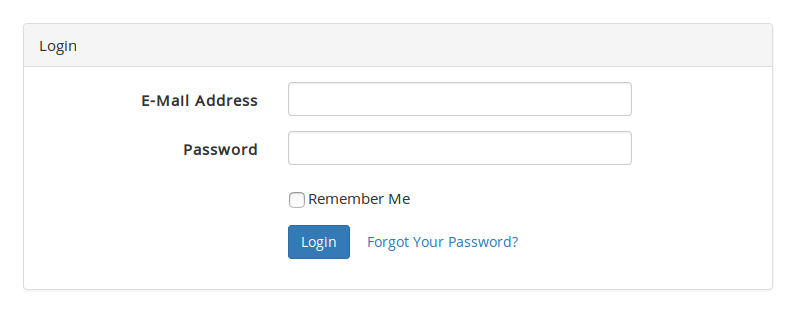
\includegraphics[scale=0.5]{login.png} \\

\vspace{0.7in}

New User Registration on Admin Panel \\
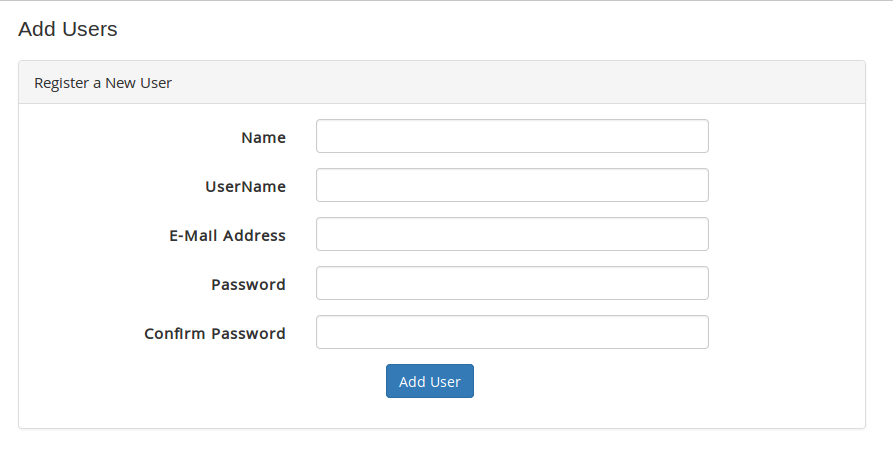
\includegraphics[scale=0.45]{user.png}	\\

\vspace{0.7in}
List of Users \\
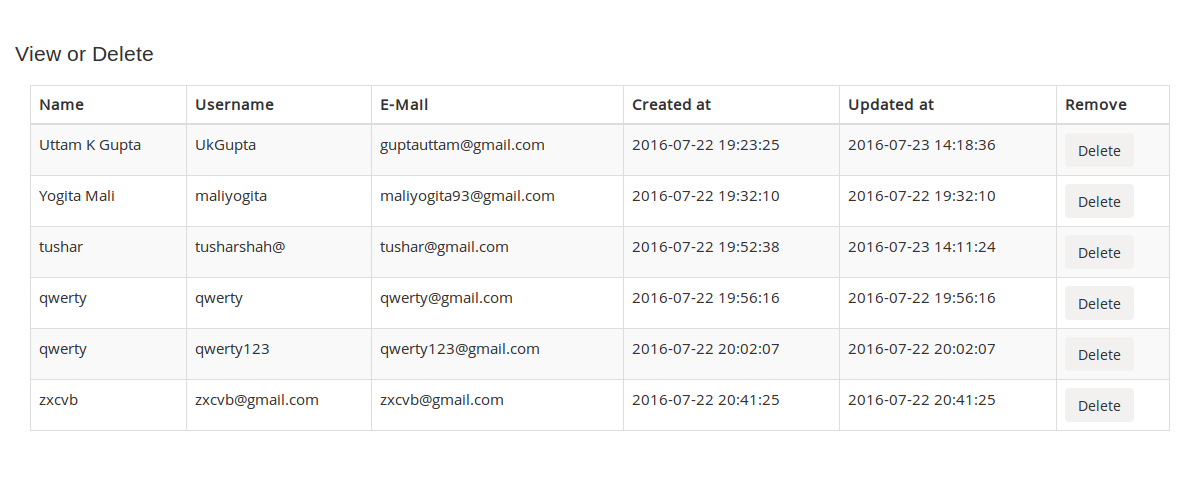
\includegraphics[scale=0.35]{user2.png}	\\

\vspace{1in}
Adding new Tags by Admin\\
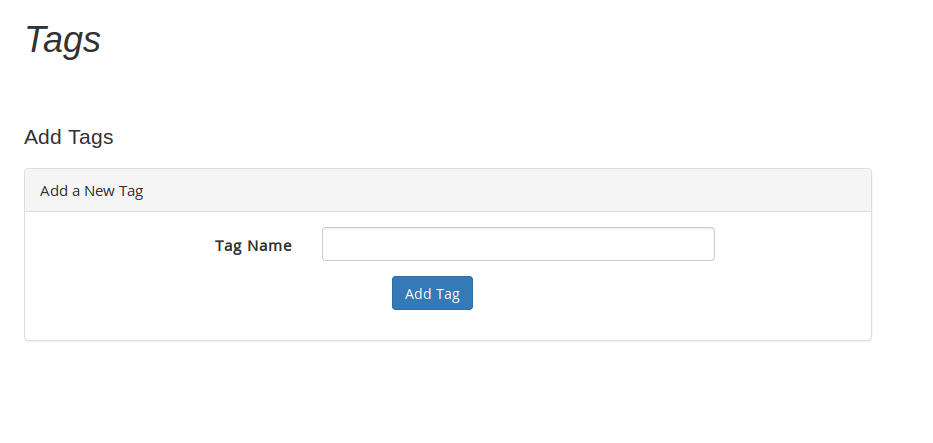
\includegraphics[scale=0.45]{tags.png}	\\

\vspace{2in}
Displaying current tags \\
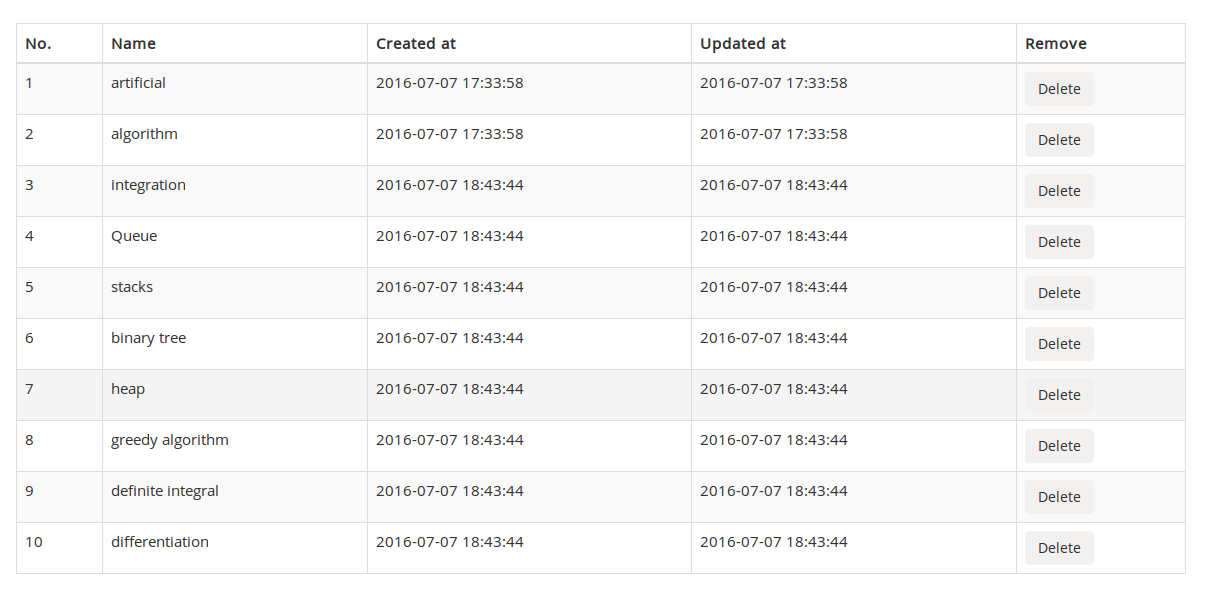
\includegraphics[scale=0.3]{tags2.png}	\\

\vspace{0.7in}
New Question for review on Admin Panel \\
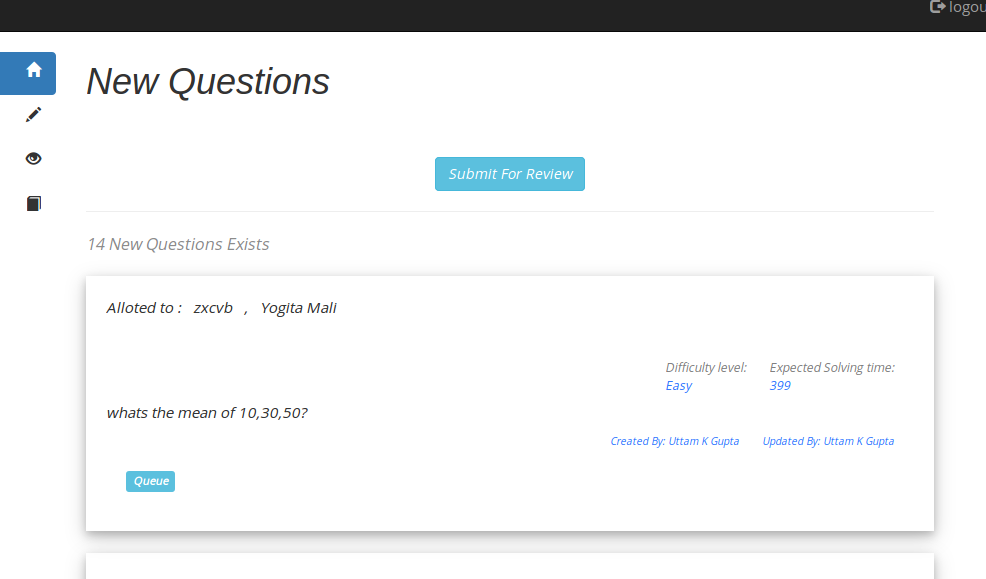
\includegraphics[scale=0.35]{newquestions.png}	\\

\vspace{2in}
Alloted or not \\
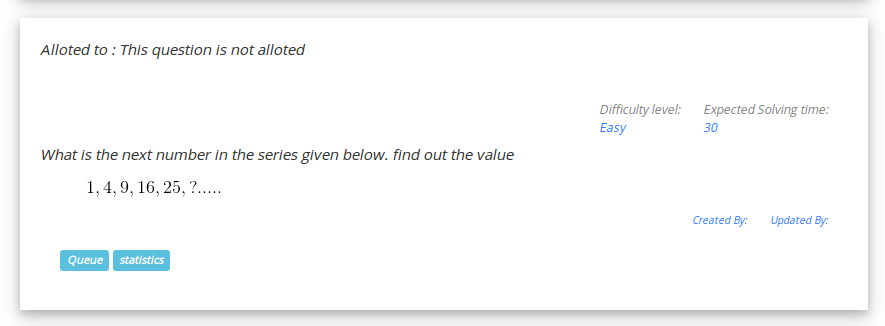
\includegraphics[scale=0.45]{alloted_unalloted.png}	\\

\vspace{1in}
Text to image conversion and options\\
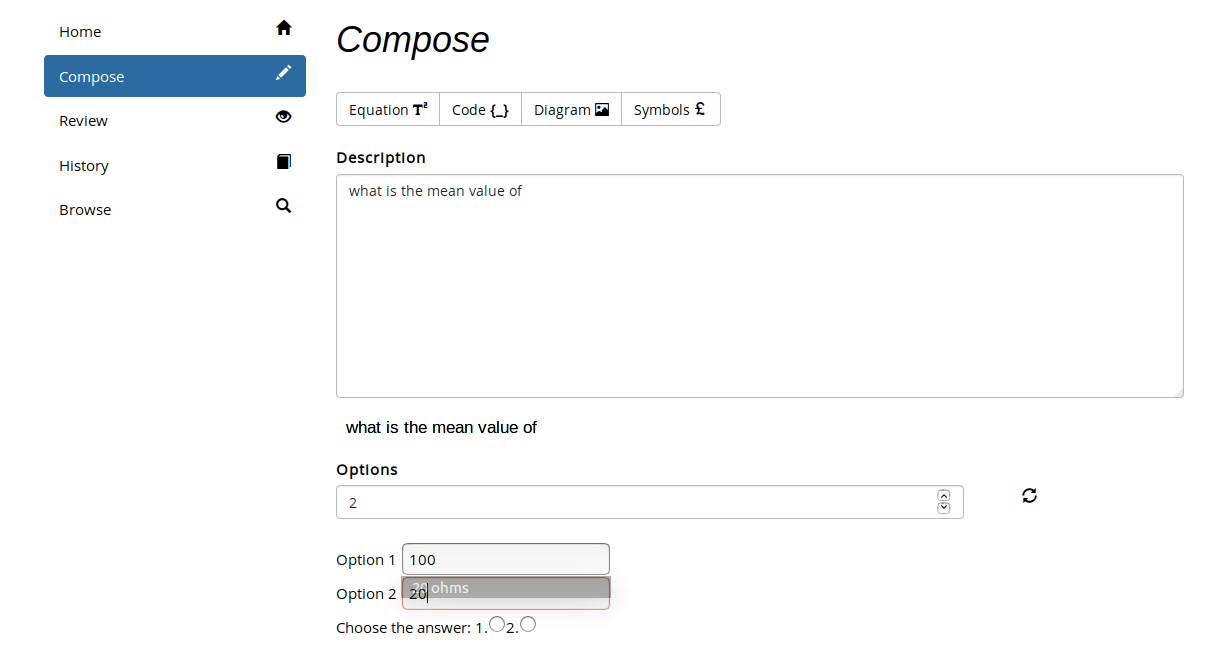
\includegraphics[scale=0.3]{compose.png}	\\

\vspace{2in}
Special Symbol keyboard\\
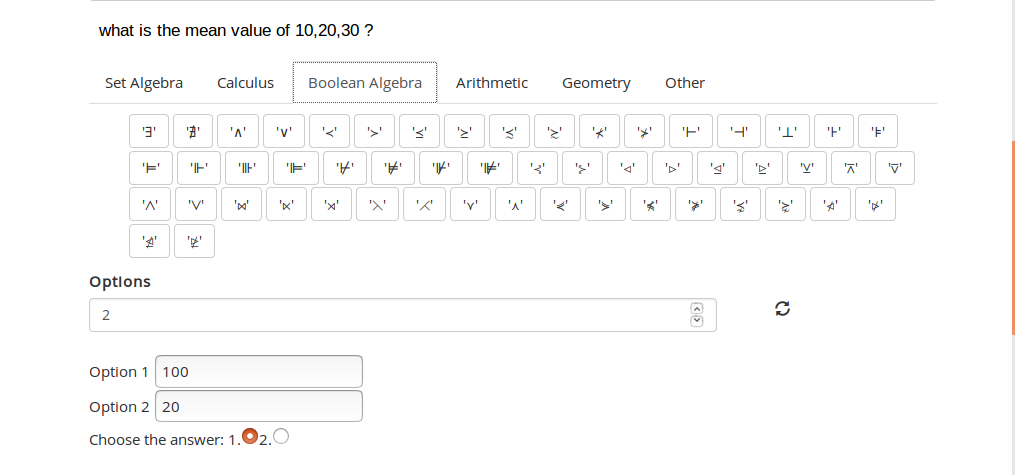
\includegraphics[scale=0.4]{compose4.png}	\\

\vspace{0.7in}
\LaTeX to image conversions\\
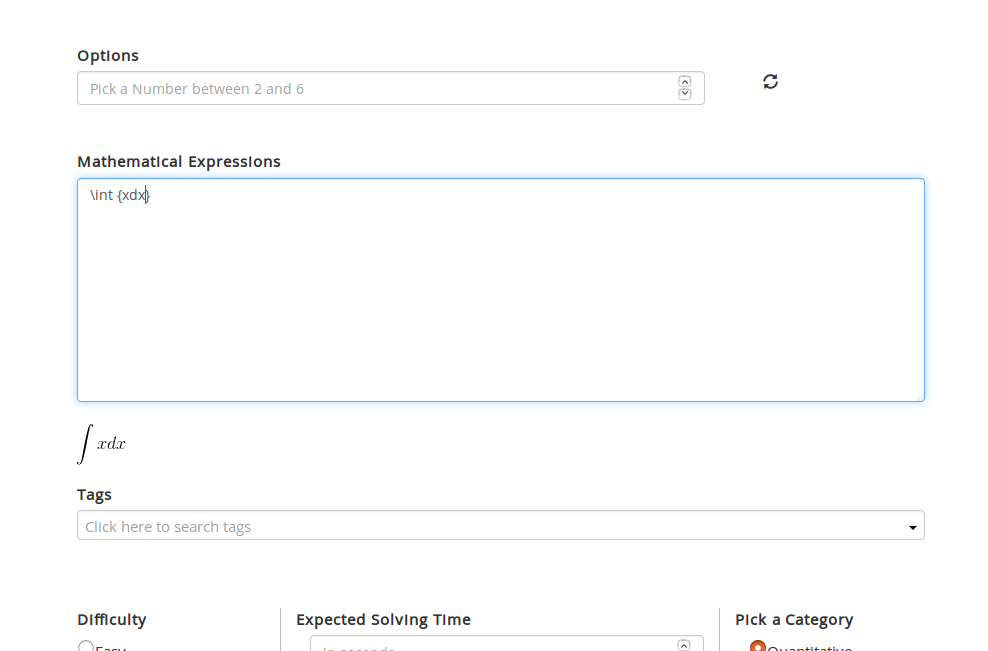
\includegraphics[scale=0.4]{compose5.png}	\\

\vspace{2in}
Code to image conversion \\
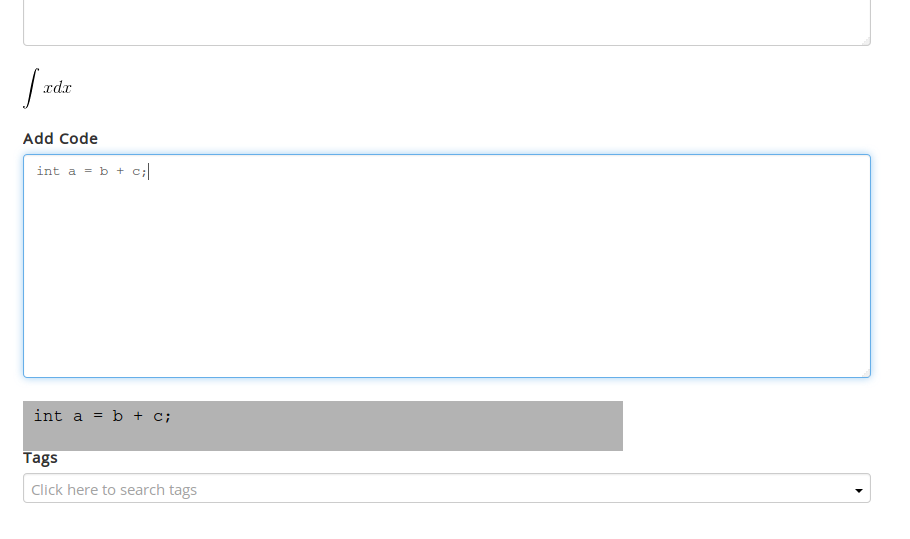
\includegraphics[scale=0.45]{compose7.png}	\\

\vspace{0.7in}
Preview of question before submit\\
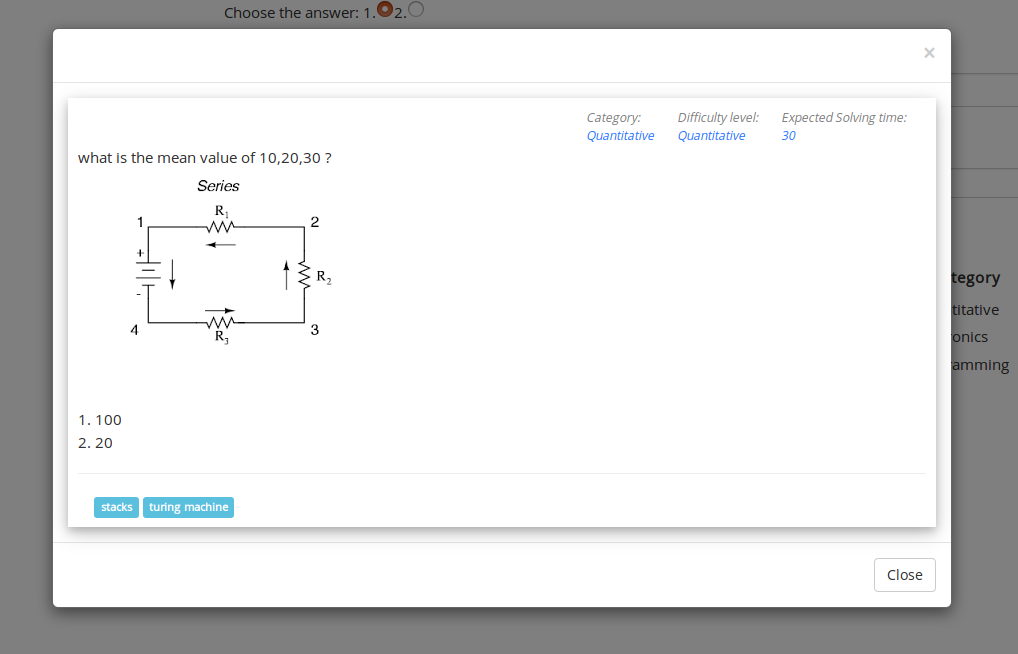
\includegraphics[scale=0.37]{preview.png}	\\

\
Browsing the question bank\\
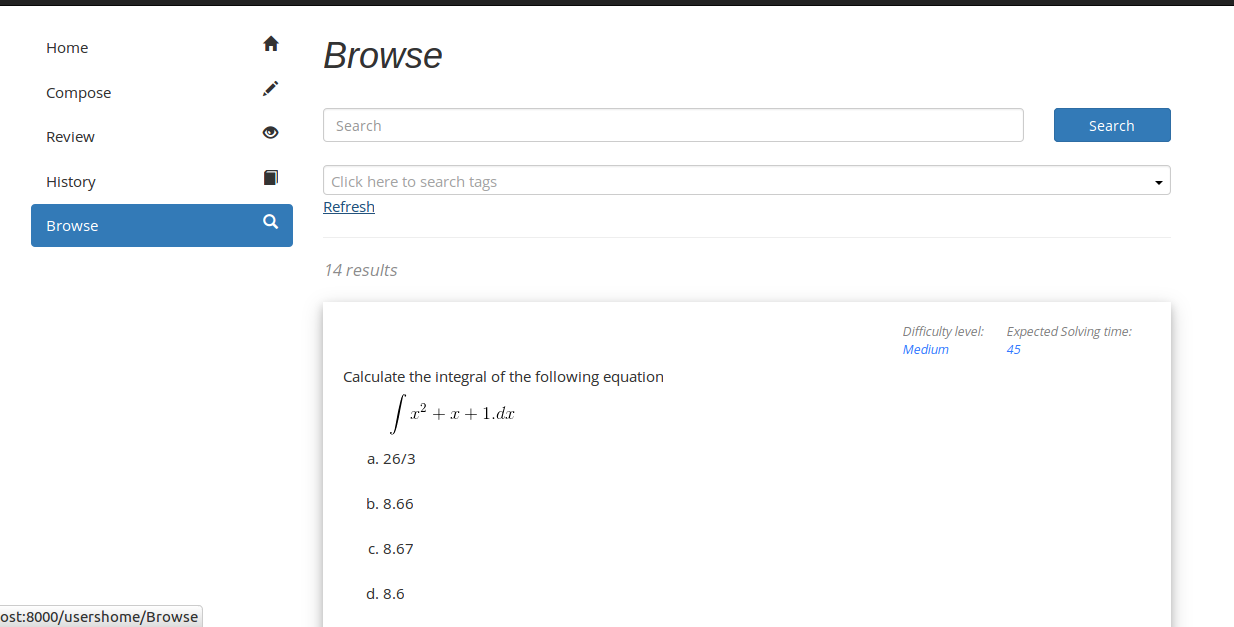
\includegraphics[scale=0.3]{browse.png}	\\

History interface\\
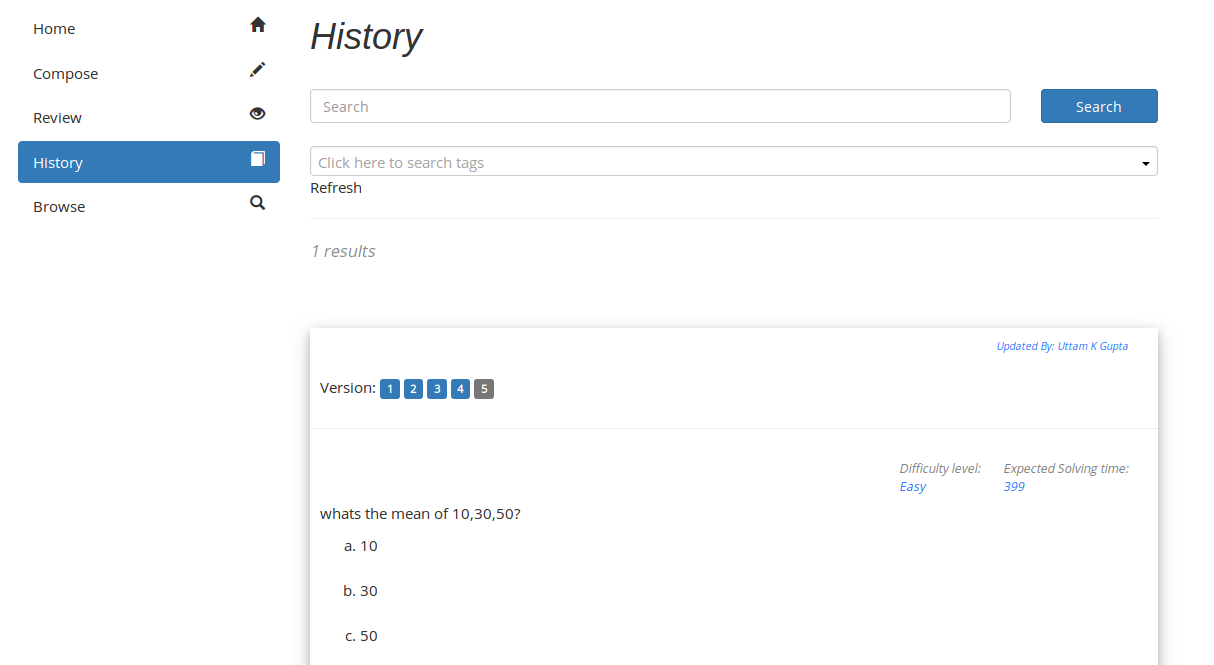
\includegraphics[scale=0.3]{history.png}	\\

\vspace{2in}
New Version \\
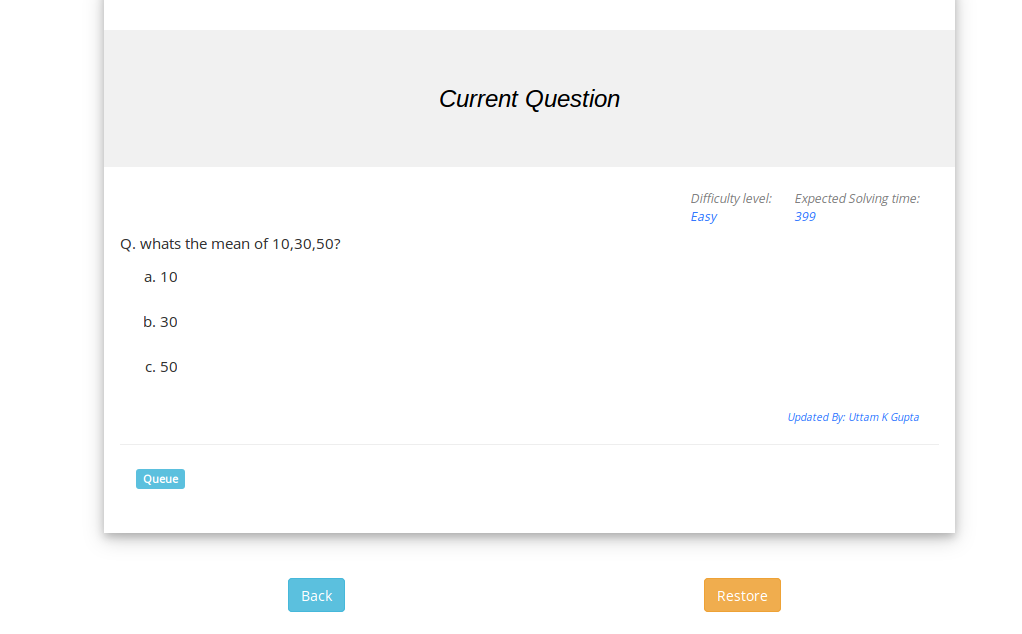
\includegraphics[scale=0.4]{version1.png}	\\

Old Version\\
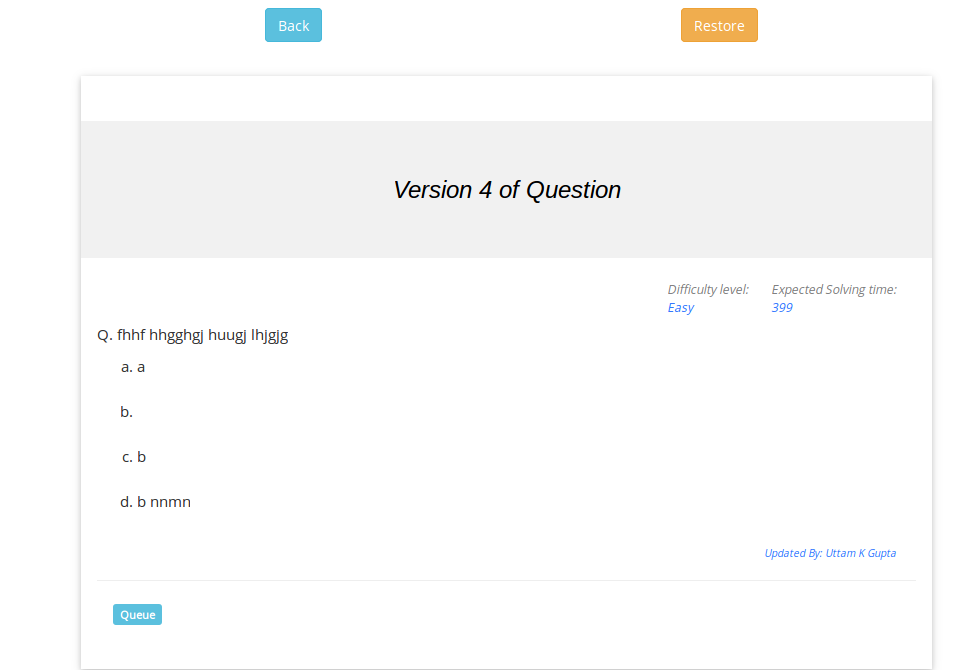
\includegraphics[scale=0.4]{version3.png}	\\

\vspace{2in}
Password Reset link \\
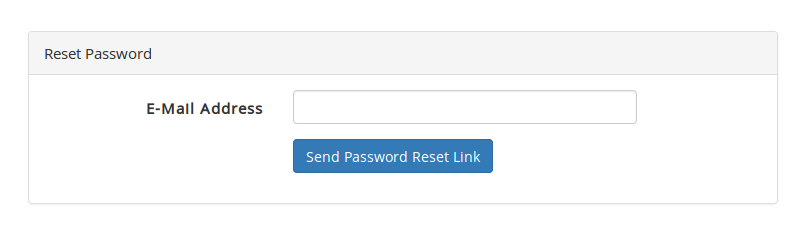
\includegraphics[scale=0.4]{password.png}	\\

\vspace{1in}
Edit a question \\
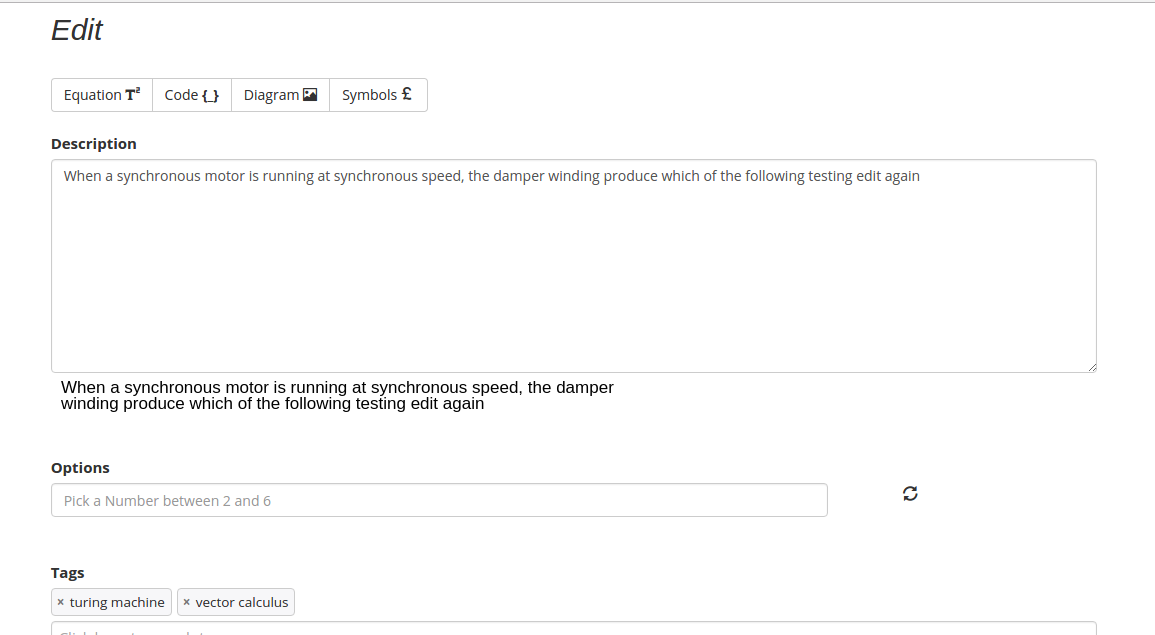
\includegraphics[scale=0.4]{edit.png}	\\

\vspace{2in}
Picking a Question \\
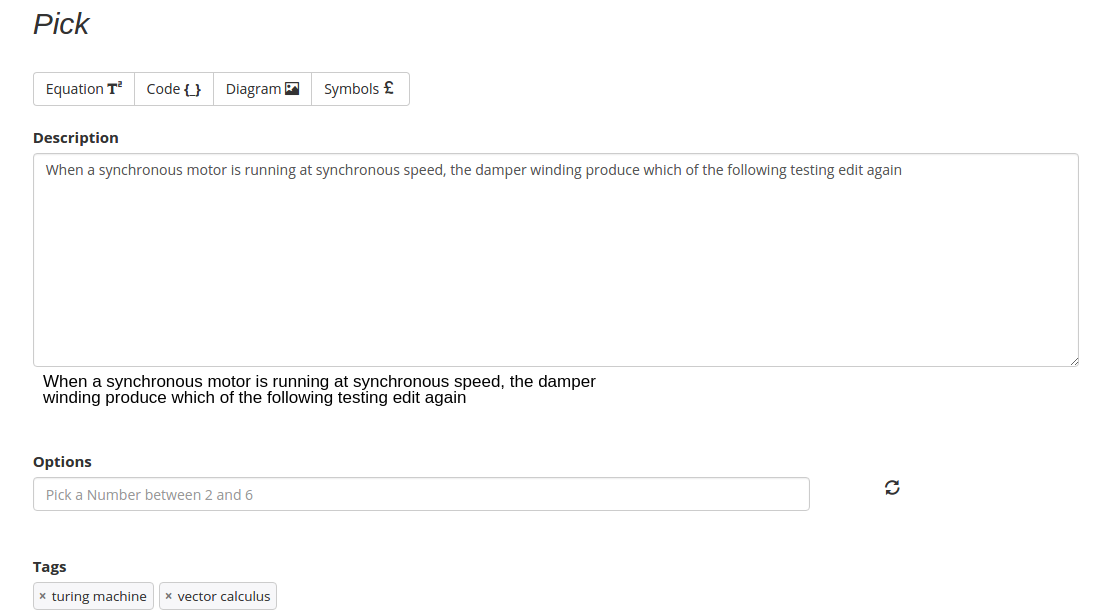
\includegraphics[scale=0.34]{pick.png}	\\

\vspace{4in}

\section{Future Work}
    \begin{itemize}
        \item Interesting insights can be gained by performing mining operations on the data generated in the system
        
        \item As every application has scope for improvement, studies can be done to develop various algorithms for distribution of questions in more selective manner and organized (as per categories or sub-categories, or difficulty level)
        
        \item The application has a coding window. APIs that give results of the code being typed and allow features such as auto-indentation can also be integrated into the existing system
        
        \item An algorithm for automating the process of creating question sets using the existing question bank can be created, each of which is of the simillar difficulty level.
    \end{itemize}

\section{Bug report and Challenges}
    \begin{itemize}
      \item Bugs
        \begin{enumerate}
          \item Small UI flaws may be present
        \end{enumerate}
      \item Challenges
           \item Designing a good UI
           \item Since the database is in the Boyce Codd Normal Form, developing efficient queries for merging data was a challenge
           \item Creating the database that shall not suffer major modifications in the long run
           \item Text to image conversion
    \end{itemize}

\begin{thebibliography}{li}
    \begin{itemize}
        \item Laravel-5.2 Documentation - \textif{https://laravel.com/docs/5.2}
        \item Stackoverflow - \textif{https://http://stackoverflow.com/}
        \item Laravel Tutorial - \textit{https://laracasts.com/series/laravel-5-from-scratch} 
        \item Laracast discussion forum - \textif{https://laracasts.com/discuss}
        \item Laravel Installation - \textif{https://www.howtoforge.com/tutorial/install-laravel-on-ubuntu-for-apache/}
        \item w3schools web tutorials series - \textif{http://www.w3schools.com/}
        \item \LaTeX equation maker API - \textif{https://www.codecogs.com/latex/eqneditor.php}
        \item Laravel Revisionable - \textif{https://github.com/VentureCraft/revisionable}
        \item Bootstrap tutorial - \textif{http://getbootstrap.com/getting-started/}
    \end{itemize}
\end{thebibliography}


\end{document}

